\documentclass[tikz,border=8pt]{standalone}
\usetikzlibrary{arrows.meta}
\begin{document}
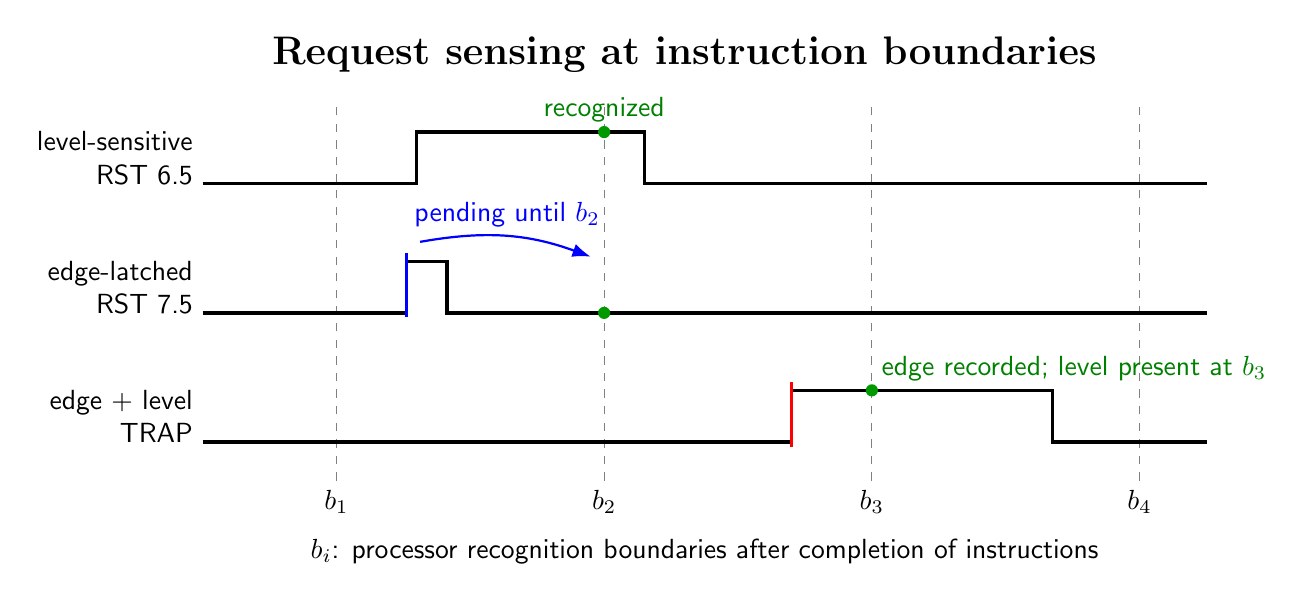
\begin{tikzpicture}[font=\sffamily,>=Latex,x=.85cm,y=.82cm]
\node[font=\Large\bfseries] at (7.2,7.25) {Request sensing at instruction boundaries};
\foreach \x/\lab in {2/$b_1$,6/$b_2$,10/$b_3$,14/$b_4$}{
  \draw[dashed,gray] (\x,.65)--(\x,6.55);
  \node[below] at (\x,.65) {\lab};
}
\node[left,align=right] at (0,5.65) {level-sensitive\\RST 6.5};
\draw[very thick] (0,5.25)--(3.2,5.25)--(3.2,6.05)--(6.6,6.05)--(6.6,5.25)--(15,5.25);
\fill[green!60!black] (6,6.05) circle (2.2pt);
\node[green!50!black,above] at (6,6.05) {recognized};

\node[left,align=right] at (0,3.65) {edge-latched\\RST 7.5};
\draw[very thick] (0,3.25)--(3.05,3.25)--(3.05,4.05)--(3.65,4.05)--(3.65,3.25)--(15,3.25);
\draw[very thick,blue] (3.05,3.18)--(3.05,4.18);
\draw[thick,blue,->] (3.25,4.35) to[bend left=15] (5.8,4.12);
\node[blue,above] at (4.55,4.43) {pending until $b_2$};
\fill[green!60!black] (6,3.25) circle (2.2pt);

\node[left,align=right] at (0,1.65) {edge + level\\TRAP};
\draw[very thick] (0,1.25)--(8.8,1.25)--(8.8,2.05)--(12.7,2.05)--(12.7,1.25)--(15,1.25);
\draw[very thick,red] (8.8,1.18)--(8.8,2.18);
\fill[green!60!black] (10,2.05) circle (2.2pt);
\node[green!50!black,above right] at (10,2.05) {edge recorded; level present at $b_3$};
\node[align=center] at (7.5,-.45) {$b_i$: processor recognition boundaries after completion of instructions};
\end{tikzpicture}
\end{document}
